\documentclass[10pt]{article}

\usepackage{polski}
\usepackage{graphicx}
\usepackage{hyperref}
\graphicspath{{images/}}

\usepackage{geometry}
\newgeometry{tmargin=4cm, bmargin=4cm, lmargin=3.2cm, rmargin=3.2cm} 

\usepackage{fancyhdr}
\pagestyle{fancy}

 

\begin{document}

% Szablon przygotowany przez Jarosława Drapałę z dalszymi zmianami Michała Karola

\begin{titlepage}
\begin{center}
  
  \LARGE \textsc{Politechnika Wrocławska}\\
  \vspace*{0.2cm}
  \Large \textsc{Wydział Informatyki i Telekomunikacji}\\  
  \vspace*{0.4cm}
  \centering
\includegraphics[width=0.2\textwidth]{images/WITlogo.png}\\
  \vspace*{0.2cm}
  \vspace*{2cm}
        
  \centerline{\rule{\textwidth}{1.2pt}}
  \vspace{0.4cm}
  \Huge\textbf{Wpływ różnych czynników na liczbę wypadków na drogach}
  \centerline{\rule{\textwidth}{1.2pt}}
  \vspace{1cm}
  \LARGE Sprawozdanie z laboratorium\\
  \vspace{3.5cm}
  \textsc{Autor}\\
  \vspace{0.2cm}
  \textbf{Paweł Wieszczeczyński}\\
  \vspace{0.1cm}
  \Large nr albumu: \textbf{260414}\\
  \vspace{0.1cm}
  kierunek: \textbf{Informatyka Stosowana}
            
            
        
        
  \vspace*{\fill}
  \Large \textit{13 czerwiec 2022}
            
 \end{center}


\end{titlepage}

\begin{abstract}
W przeprowadzonej analizie zbadano wpływ różnych czynników na ilość wypadków (zdarzenie mające związek z ruchem pojazdów na drogach publicznych, w wyniku którego nastąpiła śmierć lub uszkodzenie ciała osób) na drogach w Polsce. Dane pobrano z Głównego Urzędu Statystycznego, a dokładniej z Banku Danych Lokalnych. W analizie wykorzystano model liniowy, oraz model kwadratowy regresji. W wyniku analizy otrzymano 5 wykresów, ukazujących wpływ każdego z wybranych przeze mnie czynników na liczbę wypadków na drogach. 

\end{abstract}

\section{Wstęp -- sformułowanie problemu}
\label{sec:wstep}
Autor potrzebuje ocenić, jakie czynniki realnie wpływają na liczbę wypadków na drogach. Dzięki tej analizie, możliwa będzie zmiana niektórych czynników, tak aby w rezultacie zmniejszyć liczbę wypadków.



\section{Opis danych}
Wielkość datasetu to 17 wierszy. Są to poszczególne dane z lat 2004 - 2020. Analizie poddane zostały następujące czynniki:
\begin{enumerate}
    \item cena 0,5l wódki czystej 40 procent [zł] 
    \item wydatki budżetów województw w dziale transport i łączność [tys. zł]
    \item emisja zanieczyszczeń pyłowych z zakładów szczególnie uciążliwych [ton rocznie]
    \item cena kursu samochodowego kat. "B" [zł]
    \item liczba osób w wieku produkcyjnym (mężczyźni 18-64 lat, kobiety 18-59 lat)
\end{enumerate}

\section{Opis rozwiązania}
Z Banku Danych Lokalnych eksportowano potrzebne dane do plików MS Excel, następnie dane zostały umieszczone w Data Frame z biblioteki Pandas. Następnie dla każdego z czynników stworzono wykresy pokazujące regresję liniową i kwadratową. Użyte zostały LinearRegresion z biblioteki sklearn, oraz model oparty na optimize.curve\_fit pokazany na laboratoriach.


\section{Rezultaty obliczeń}

\subsection{Plan badań}
Zbiór danych zostanie podzielony na dwie części: treningową i testową w stosunku 80:20. 
\pagebreak

\subsection{Wyniki obliczeń}

\subsubsection{Cena wódki}
\begin{figure}[h]
\begin{center}
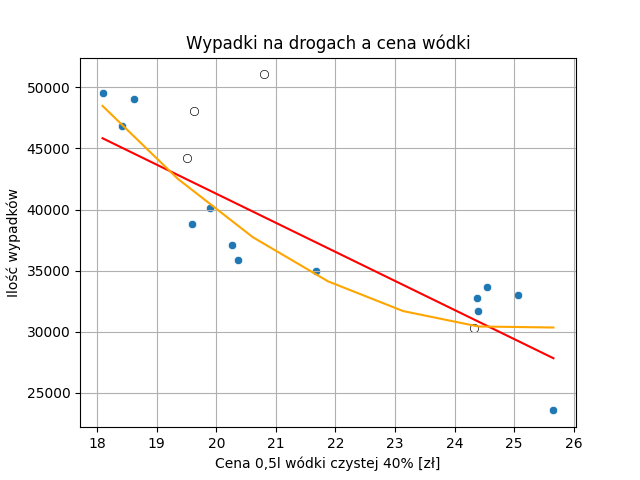
\includegraphics[width=0.5\linewidth]{images/plots/wodka.png}
\caption{Wypadki na drogach a cena wódki}
\end{center}
\end{figure}
Jak można zauważyć na wykresie, wraz ze wzrostem cen wódki, znacznie maleje ilość wypadków na drogach (stromy wykres liniowy). Analizując regresję kwadratową, można również zauważyć, że ilość wypadków spada bardzo szybko kiedy ceny wódki rosną z niskich wartości. Kiedy wódka jest droga, wzrost ceny nie powoduje już tak dużego zmniejszenia wypadków na drogach. 

\subsubsection{Wydatki województw}
\begin{figure}[h]
\begin{center}
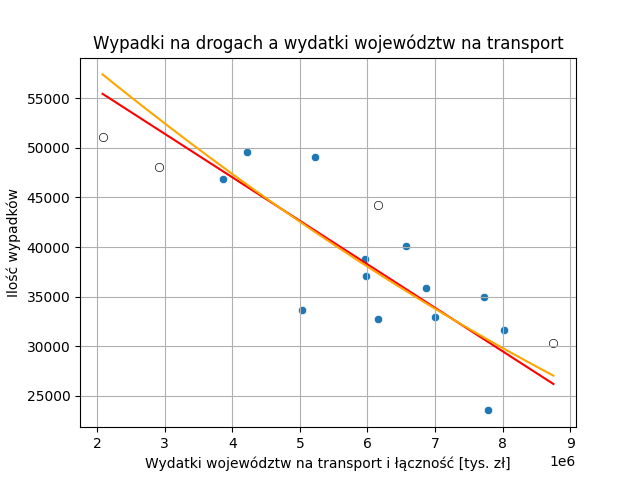
\includegraphics[width=0.5\linewidth]{images/plots/woj.png}
\caption{Wypadki na drogach a wydatki województw na transport}
\end{center}
\end{figure}
Ponownie, zwiększenie badanego czynnika znacząco redukuje ilość wypadków na drogach. Co ciekawe, regresja liniowa jak i kwadratowa wyglądają praktycznie tak samo, co oznacza, że już model liniowy, relatywnie dobrze opisuje zależność pomiędzy wypadkami a wydatkami województw

\subsubsection{Emisja zanieczyszczeń}
\begin{figure}[h]
\begin{center}
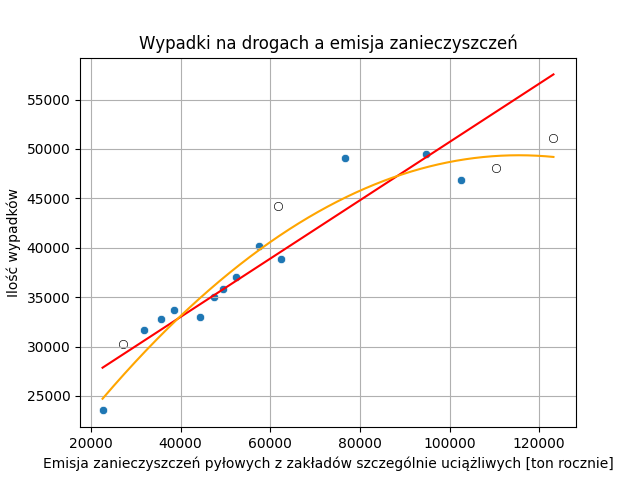
\includegraphics[width=0.5\linewidth]{images/plots/emisja.png}
\caption{Wypadki na drogach a emisja zanieczyszczeń}
\end{center}
\end{figure}
W tym przypadku zależność jest odwrotna. Zwiększenie emisji zanieczyszczeń pyłowych w zakładach szczególnie uciążliwych zwiększa ilość wypadków na Polskich drogach. Dzięki regresji kwadratowej, można zauważyć że najszybciej liczba wypadków rośnie kiedy emisja zanieczyszczeń jest niska. Kiedy emisja jest wysoka, dodatkowe jej zwiększenie nie wpływa już tak mocno na ilość wypadków.

\subsubsection{Cena kursu kat. "B"}
\begin{figure}[h]
\begin{center}
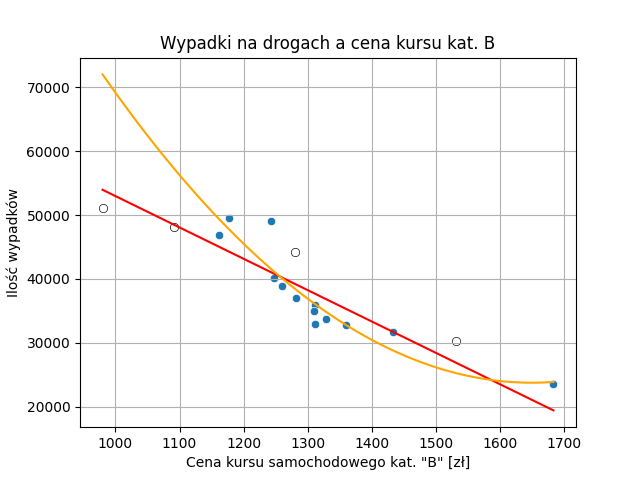
\includegraphics[width=0.5\linewidth]{images/plots/kurs.png}
\caption{Wypadki na drogach a cena kursu kat. "B"}
\end{center}
\end{figure}
Jak można zauważyć na wykresie, wraz ze wzrostem cen kursu kat. "B", zmniejsza się ilość wypadków na drogach. Jest to niezgodne z logiką, zatem warto wspomnieć, że analizowane są jedynie suche, wybiórcze dane, a w rzeczywistości, na ilość wypadków wpływa kombinacja bardzo wielu czynników. Jednak według regresji zarówno liniowej jak i kwadratowej, na zmniejszenie ilości wypadków wpływ może mieć zmniejszenie cen kursu kat. "B".

\subsubsection{Liczba osób w wieku produkcyjnym}
\begin{figure}[h]
\begin{center}
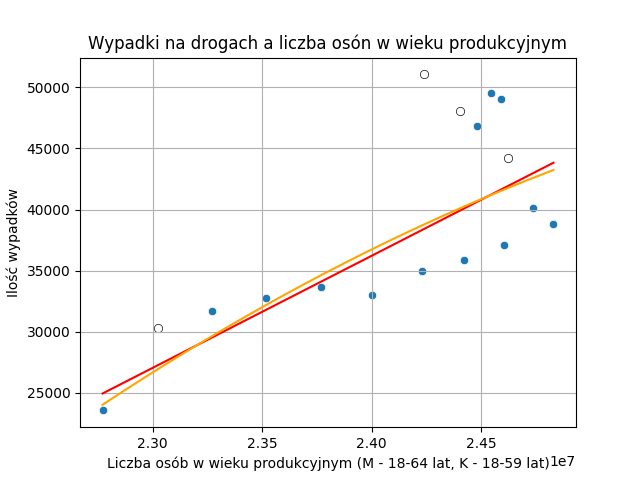
\includegraphics[width=0.5\linewidth]{images/plots/ludzie.png}
\caption{Wypadki na drogach a liczba osób w wieku produkcyjnym}
\end{center}
\end{figure}
Jak pokazuje ostatni wykres, wraz ze wzrostem liczby osób w wieku produkcyjnym, rośnie również liczba wypadków. Ponownie, wykres regresji kwadratowej jest niemalże taki sam jak regresji liniowej.

\section{Wnioski}
Pokazane na wykresach zależności pokazują, że liczbę wypadków można skojarzyć z wieloma czynnikami. Zazwyczaj najwiekszy wpływ mają zmiany przy danych które są relatywnie niższe od reszty danych. Większość z przeanalizowanych zależności ma sens. 

Jeśli chodzi o cenę wódki, to jej wzrost może znacząco wpływać na zmniejszenie liczby wypadków, przez to, że w Polsce jest duży problem z kierowaniem pod wpływem alkoholu. Wyższe ceny sprawiają, że mniej wódki jest kupowane, a co za tym idzie być może mniej osób kieruje po pijaku.

W przypadku liczby osób w wieku produkcyjnym, to liczba ta bezpośrednio przekłada się na liczbę samochodów na drogach. Więcej ludzi dojeżdząjących do pracy - więcej samochodów, więcej samochodów - więcej wypadków.

Wydatki województw na transport i łączność bezpośrednio wpływają na insfrastrukturę drogową w Polsce, co przekłada się na bezpieczeństwo i mniejsze szanse na zdażenie się wypadku.

Negatywnie z kolei wpływa zwiększenie emisji zanieczyszczeń pyłowych. Również to jest prawdopodobne, gdyż ilość zanieczyszczeń pyłowych może ograniczać widoczność, co zmniejsza bezpieczeństwo na drogach i może zwiększyć szanse na wypadek.

Nielogiczne są natomiast wnioski z analizy cen kursu kat. "B" i ilości wypadków na drogach. Jak się okazuje, im droższy jest owy kurs, tym mniej wypadków na drogach. Skoro jest on droższy, to zwiększa się szansa, że ludzi nie będzie stać na owy kurs, a co za tym idzie, mogą oni być skłonni do kierowania samochodem bez odpowiednich umiejętności, powodując tym samym więcej wypadków. Być może jednak zwiększenie cen, zmniejsza samą ilość kierowców, gdyż nie chcą oni wydawać tak dużej ilości pieniędzy na próbę zdania egzaminu na prawo jazdy.

Przedstawiona analiza może pozytywnie wpłynąć na zmniejszenie ilości wypadków na drogach. Przykładowo zarządy województw mogą przeznaczać więcej pieniędzy na transport i łączność, gdyż lepsza infrastruktura może zwiększyć bezpieczeństwo na drogach. Analogicznie, kiedy podniesione zostaną ceny wódki, jest bardzo duża szansa na to, że wraz z konsumpcją wódki, zmniejszy się również ilość wypadków. Model ten jest jednak dużym uproszczeniem i w rzeczywistości na liczbę wypadków drogowych ma wpływ jeszcze wiele innych czynników. 

\appendix
\section{Dodatek}
Kod źródłowy został umieszczony w repozytorium na github.com.

\noindent \url{https://github.com/PawelWieszczeczynski/MSiD_Projekt}.


\end{document}